\documentclass[lesson_slides]{subfiles}
\usepackage{natbib}
\usepackage{graphicx}
% \graphicspath{ {./images/} }
\usepackage{enumerate}
\usepackage{pifont} % for ding
\usepackage{float} % keeps tables in the exact position they occupy in the code
\usepackage{xcolor} % text colour
\usepackage{gb4e} % leave last

\begin{document}
%%=-=-=-=-=-=-=-=-=-=-=-=-=-=-=-=-=-=-=-=-=-=-=-=-=-=-=-=-=-=-=-=-=-=-=-=-=-=-=-=
%   FRAME START   -=-=-=-=-=-=-=-=-=-=-=-=-=-=-=-=-=-=-=-=-=-=-=-=-=-=-=-=-=-=-=
\begin{frame}[c]{French wh-interrogatives from 1870 to 2014}

    \begin{center}
        \textbf{How have French interrogatives evolved between 1870 and 2014?}
    \end{center}
  
\end{frame}
%   FRAME END   --==-=-=-=-=-=-=-=-=-=-=-=-=-=-=-=-=-=-=-=-=-=-=-=-=-=-=-=-=-=-=
%   FRAME START   -=-=-=-=-=-=-=-=-=-=-=-=-=-=-=-=-=-=-=-=-=-=-=-=-=-=-=-=-=-=-=
\begin{frame}[c]{French wh-interrogatives from 1870 to 2014}
    
    \transboxin<1>
        \transglitter<2>
        \transwipe<3>
        We observed three main evolutions: \pause 
        \begin{itemize}
            \item[\ding{227}] from \underline{predominant phrasal} movement to predominant non movement of phrases;\\ \pause $\longrightarrow$ wh-ex situ to wh-in situ. \pause
            \item[\ding{227}] from verb movement and head activation to predominant non-movement/activation;\\ \pause $\longrightarrow$ from VS to SV. \pause
            \item[\ding{227}] from head activation to predominant non-activation.\\ \pause $\longrightarrow$ from 'est-ce que' to SV.
        \end{itemize}
  
\end{frame}
%   FRAME END   --==-=-=-=-=-=-=-=-=-=-=-=-=-=-=-=-=-=-=-=-=-=-=-=-=-=-=-=-=-=-=
%   FRAME START   -=-=-=-=-=-=-=-=-=-=-=-=-=-=-=-=-=-=-=-=-=-=-=-=-=-=-=-=-=-=-=
\begin{frame}[c]{From predominant wh-ex situ to predominant wh-in situ}

\textbf{\textsc{our raw data}}

\begin{table}[H]
    \centering
    \small
    \begin{adjustbox}
        \begin{tabular}{l|rr|rr|rr|rr|rr}
        % \hline
        {} & \multicolumn{2}{c}{comment}  & \multicolumn{2}{c}{où} & \multicolumn{2}{c}{quand} & \multicolumn{2}{c}{quiO}& \multicolumn{2}{c}{quoiO}\\
        \hline
        {} & EX & IN & EX & IN & EX & IN & EX & IN & EX & IN\\
        %\hline
        1870$-$1900 & 60 & 0 & 102 & 0 & 14 & 0 & 15 & 0 & 36 & 0\\
        %\hline
        1900$-$1930 & 40 & 0 & 39 & 0 & 4 & 0 & 9 & 0 & 17 & 0\\
        %\hline
        1970 (eslo 1) & 848 & 37 & 233 & 72 & 156 & 38 & 42 & 13 & 333 & 198\\
        %\hline
        2014 (eslo 2) & 333 & 156 & 84 & 260 & 32 & 30 & 8 & 21 & 24 & 476 \\
        \hline
        \end{tabular}
    \end{adjustbox}
\caption{\label{tab:samp3}Total occurrences of non lexically-restricted wh-elements.}
\end{table}
  
\end{frame}
%   FRAME END   --==-=-=-=-=-=-=-=-=-=-=-=-=-=-=-=-=-=-=-=-=-=-=-=-=-=-=-=-=-=-=
%   FRAME START   -=-=-=-=-=-=-=-=-=-=-=-=-=-=-=-=-=-=-=-=-=-=-=-=-=-=-=-=-=-=-=
\begin{frame}[c]{From predominant wh-ex situ to predominant wh-in situ}

\textbf{\textsc{our raw data}}

\begin{table}[H]
    \centering
    \small
    \begin{adjustbox}
        \begin{tabular}{l|rr|rr|rr|rr|rr}
        % \hline
        {} & \multicolumn{2}{c}{comment}  & \multicolumn{2}{c}{où} & \multicolumn{2}{c}{quand} & \multicolumn{2}{c}{quiO}& \multicolumn{2}{c}{quoiO}\\
        \hline
        {} & EX & IN & EX & IN & EX & IN & EX & IN & EX & IN\\
        %\hline
        \hl{1870$-$1900} & 60 & 0 & 102 & 0 & 14 & 0 & 15 & 0 & 36 & 0\\
        %\hline
        \hl{1900$-$1930} & 40 & 0 & 39 & 0 & 4 & 0 & 9 & 0 & 17 & 0\\
        %\hline
        1970 (eslo 1) & 848 & 37 & 233 & 72 & 156 & 38 & 42 & 13 & 333 & 198\\
        %\hline
        2014 (eslo 2) & 333 & 156 & 84 & 260 & 32 & 30 & 8 & 21 & 24 & 476 \\
        \hline
        \end{tabular}
    \end{adjustbox}
\caption{\label{tab:samp3}Total occurrences of non lexically-restricted wh-elements.}
\end{table}
  
\end{frame}
%   FRAME END   --==-=-=-=-=-=-=-=-=-=-=-=-=-=-=-=-=-=-=-=-=-=-=-=-=-=-=-=-=-=-=
%   FRAME START   -=-=-=-=-=-=-=-=-=-=-=-=-=-=-=-=-=-=-=-=-=-=-=-=-=-=-=-=-=-=-=
\begin{frame}[c]{From predominant wh-ex situ to predominant wh-in situ}

\begin{table}[H]
    \centering
    \small
    \begin{adjustbox}
        \begin{tabular}{l|rr|rr|rr|rr|rr}
        % \hline
        {} & \multicolumn{2}{c}{comment}  & \multicolumn{2}{c}{où} & \multicolumn{2}{c}{quand} & \multicolumn{2}{c}{quiO}& \multicolumn{2}{c}{quoiO}\\
        \hline
        {} & EX & \hl{IN} & EX & \hl{IN} & EX & \hl{IN} & EX & \hl{IN} & EX & \hl{IN}\\
        %\hline
        \hl{1870$-$1900} & 60 & 0 & 102 & 0 & 14 & 0 & 15 & 0 & 36 & 0\\
        %\hline
        \hl{1900$-$1930} & 40 & 0 & 39 & 0 & 4 & 0 & 9 & 0 & 17 & 0\\
        %\hline
        1970 (eslo 1) & 848 & 37 & 233 & 72 & 156 & 38 & 42 & 13 & 333 & 198\\
        %\hline
        2014 (eslo 2) & 333 & 156 & 84 & 260 & 32 & 30 & 8 & 21 & 24 & 476 \\
        \hline
        \end{tabular}
    \end{adjustbox}
\caption{\label{tab:samp3}Total occurrences of non lexically-restricted wh-elements.}
\end{table}
  
\end{frame}
%   FRAME END   --==-=-=-=-=-=-=-=-=-=-=-=-=-=-=-=-=-=-=-=-=-=-=-=-=-=-=-=-=-=-=
%   FRAME START   -=-=-=-=-=-=-=-=-=-=-=-=-=-=-=-=-=-=-=-=-=-=-=-=-=-=-=-=-=-=-=
\begin{frame}[c]{From predominant wh-ex situ to predominant wh-in situ}

\begin{table}[H]
    \centering
    \small
    \begin{adjustbox}
        \begin{tabular}{l|rr|rr|rr|rr|rr}
        % \hline
        {} & \multicolumn{2}{c}{comment}  & \multicolumn{2}{c}{où} & \multicolumn{2}{c}{quand} & \multicolumn{2}{c}{quiO}& \multicolumn{2}{c}{quoiO}\\
        \hline
        {} & EX & \hl{IN} & EX & \hl{IN} & EX & \hl{IN} & EX & \hl{IN} & EX & \hl{IN}\\
        %\hline
        \hl{1870$-$1900} & 60 & \textcolor{red}{0} & 102 & \textcolor{red}{0} & 14 & \textcolor{red}{0} & 15 & \textcolor{red}{0} & 36 & \textcolor{red}{0}\\
        %\hline
        \hl{1900$-$1930} & 40 & \textcolor{red}{0} & 39 & \textcolor{red}{0} & 4 & \textcolor{red}{0} & 9 & \textcolor{red}{0} & 17 & \textcolor{red}{0}\\
        %\hline
        1970 (eslo 1) & 848 & 37 & 233 & 72 & 156 & 38 & 42 & 13 & 333 & 198\\
        %\hline
        2014 (eslo 2) & 333 & 156 & 84 & 260 & 32 & 30 & 8 & 21 & 24 & 476 \\
        \hline
        \end{tabular}
    \end{adjustbox}
\caption{\label{tab:samp3}Total occurrences of non lexically-restricted wh-elements.}
\end{table}
  
\end{frame}
%   FRAME END   --==-=-=-=-=-=-=-=-=-=-=-=-=-=-=-=-=-=-=-=-=-=-=-=-=-=-=-=-=-=-=
%   FRAME START   -=-=-=-=-=-=-=-=-=-=-=-=-=-=-=-=-=-=-=-=-=-=-=-=-=-=-=-=-=-=-=
\begin{frame}[c]{From predominant wh-ex situ to predominant wh-in situ}

    \transboxin<1>
    \transglitter<2>
    %\transwipe<3>
    \textbf{\textsc{the decline of wh-ex situ}} \pause (all types combined) \pause
    \begin{center}
        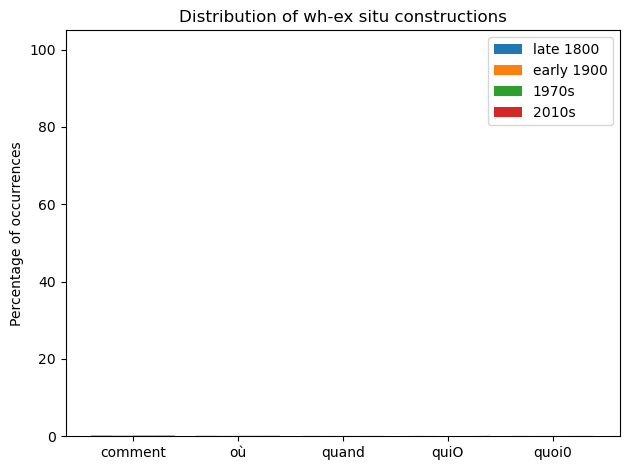
\includegraphics[width=10cm, height=6cm]{images/exsitu.png}
    \end{center}
  
\end{frame}
%   FRAME END   --==-=-=-=-=-=-=-=-=-=-=-=-=-=-=-=-=-=-=-=-=-=-=-=-=-=-=-=-=-=-=
%   FRAME START   -=-=-=-=-=-=-=-=-=-=-=-=-=-=-=-=-=-=-=-=-=-=-=-=-=-=-=-=-=-=-=
\begin{frame}[c]{From predominant wh-ex situ to predominant wh-in situ}

    \textbf{\textsc{the decline of wh-ex situ}} (all types combined)
    \begin{center}
        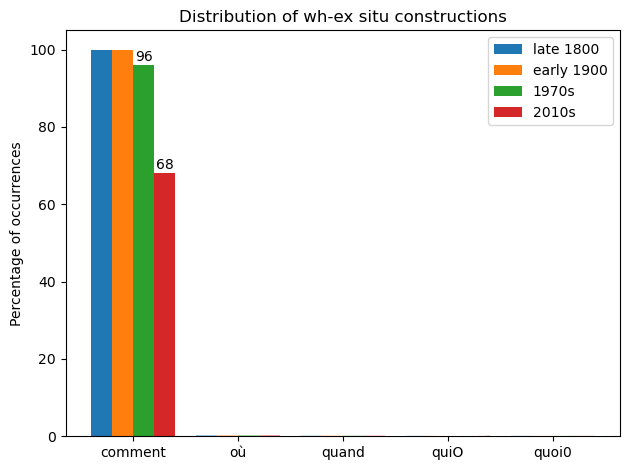
\includegraphics[width=10cm, height=6cm]{images/exsitu1.png}
    \end{center}
  
\end{frame}
%   FRAME END   --==-=-=-=-=-=-=-=-=-=-=-=-=-=-=-=-=-=-=-=-=-=-=-=-=-=-=-=-=-=-=
%   FRAME START   -=-=-=-=-=-=-=-=-=-=-=-=-=-=-=-=-=-=-=-=-=-=-=-=-=-=-=-=-=-=-=
\begin{frame}[c]{From predominant wh-ex situ to predominant wh-in situ}

    \textbf{\textsc{the decline of wh-ex situ}} (all types combined)
    \begin{center}
        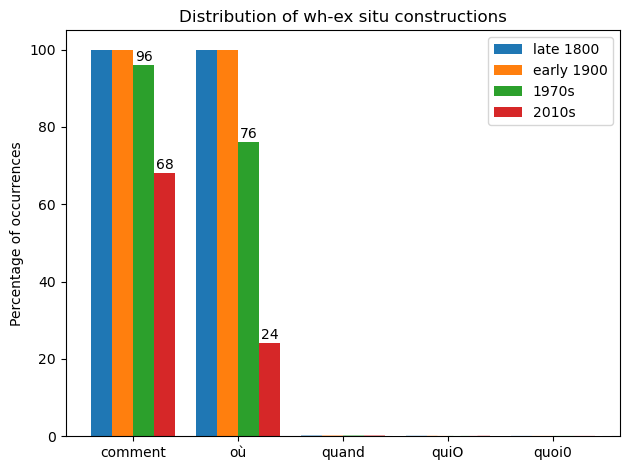
\includegraphics[width=10cm, height=6cm]{images/exsitu2.png}
    \end{center}
  
\end{frame}
%   FRAME END   --==-=-=-=-=-=-=-=-=-=-=-=-=-=-=-=-=-=-=-=-=-=-=-=-=-=-=-=-=-=-=
%   FRAME START   -=-=-=-=-=-=-=-=-=-=-=-=-=-=-=-=-=-=-=-=-=-=-=-=-=-=-=-=-=-=-=
\begin{frame}[c]{From predominant wh-ex situ to predominant wh-in situ}

    \textbf{\textsc{the decline of wh-ex situ}} (all types combined)
    \begin{center}
        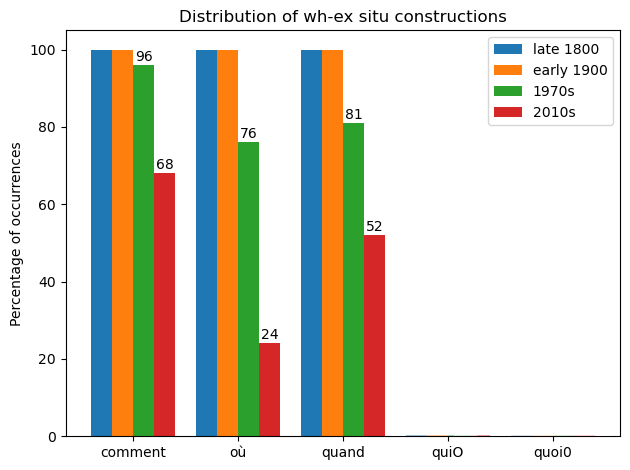
\includegraphics[width=10cm, height=6cm]{images/exsitu3.png}
    \end{center}
  
\end{frame}
%   FRAME END   --==-=-=-=-=-=-=-=-=-=-=-=-=-=-=-=-=-=-=-=-=-=-=-=-=-=-=-=-=-=-=
%   FRAME START   -=-=-=-=-=-=-=-=-=-=-=-=-=-=-=-=-=-=-=-=-=-=-=-=-=-=-=-=-=-=-=
\begin{frame}[c]{From predominant wh-ex situ to predominant wh-in situ}

    \textbf{\textsc{the decline of wh-ex situ}} (all types combined)
    \begin{center}
        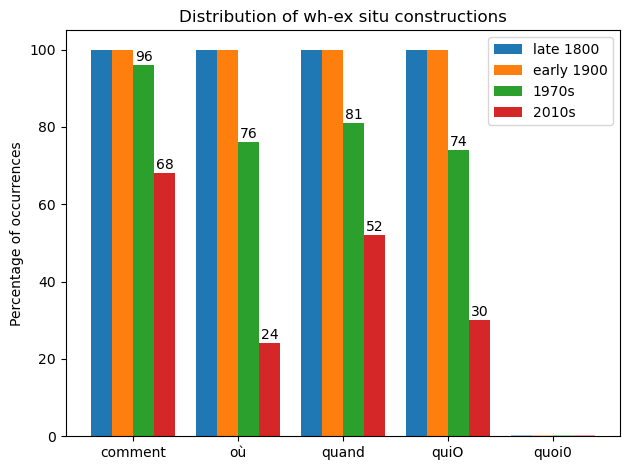
\includegraphics[width=10cm, height=6cm]{images/exsitu4.png}
    \end{center}
  
\end{frame}
%   FRAME END   --==-=-=-=-=-=-=-=-=-=-=-=-=-=-=-=-=-=-=-=-=-=-=-=-=-=-=-=-=-=-=
%   FRAME START   -=-=-=-=-=-=-=-=-=-=-=-=-=-=-=-=-=-=-=-=-=-=-=-=-=-=-=-=-=-=-=
\begin{frame}[c]{From predominant wh-ex situ to predominant wh-in situ}

    \textbf{\textsc{the decline of wh-ex situ}} (all types combined)
    \begin{center}
        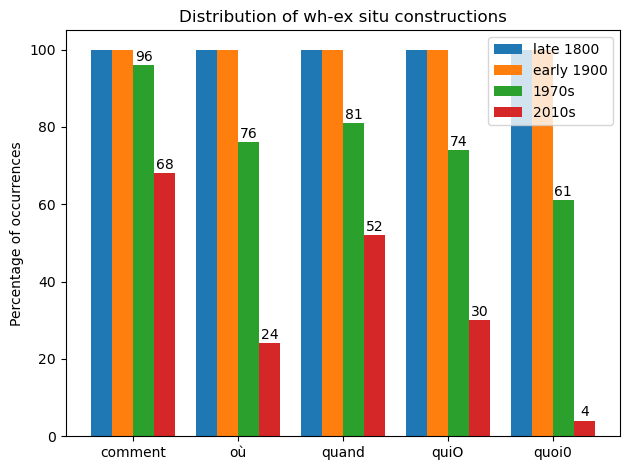
\includegraphics[width=10cm, height=6cm]{images/exsitu5.png}
    \end{center}
  
\end{frame}
%   FRAME END   --==-=-=-=-=-=-=-=-=-=-=-=-=-=-=-=-=-=-=-=-=-=-=-=-=-=-=-=-=-=-=
%   FRAME START   -=-=-=-=-=-=-=-=-=-=-=-=-=-=-=-=-=-=-=-=-=-=-=-=-=-=-=-=-=-=-=
\begin{frame}[c]{From predominant wh-ex situ to predominant wh-in situ}

\begin{center}
    \textbf{Let's try to see this in a clearer way...}
\end{center}
  
\end{frame}
%   FRAME END   --==-=-=-=-=-=-=-=-=-=-=-=-=-=-=-=-=-=-=-=-=-=-=-=-=-=-=-=-=-=-=
%   FRAME START   -=-=-=-=-=-=-=-=-=-=-=-=-=-=-=-=-=-=-=-=-=-=-=-=-=-=-=-=-=-=-=
\begin{frame}[c]{From predominant wh-ex situ to predominant wh-in situ}

    \transboxin<1>
    \transglitter<2>
    %\transwipe<3>
    \textbf{\textsc{the decline of wh-ex situ}} \pause (all types combined) \pause
    \begin{center}
        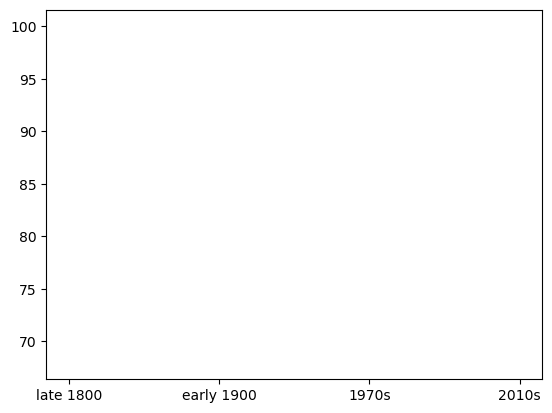
\includegraphics[width=10cm, height=6cm]{images/empty.png}
    \end{center}
  
\end{frame}
%   FRAME END   --==-=-=-=-=-=-=-=-=-=-=-=-=-=-=-=-=-=-=-=-=-=-=-=-=-=-=-=-=-=-=
%   FRAME START   -=-=-=-=-=-=-=-=-=-=-=-=-=-=-=-=-=-=-=-=-=-=-=-=-=-=-=-=-=-=-=
\begin{frame}[c]{From predominant wh-ex situ to predominant wh-in situ}

    \textbf{\textsc{the decline of wh-ex situ}} (all types combined)
    \begin{center}
        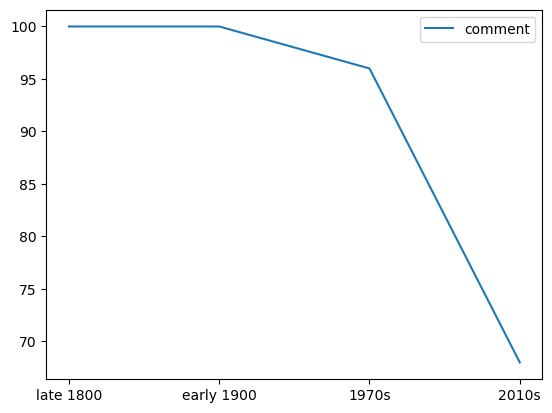
\includegraphics[width=10cm, height=6cm]{images/one.png}
    \end{center}
  
\end{frame}
%   FRAME END   --==-=-=-=-=-=-=-=-=-=-=-=-=-=-=-=-=-=-=-=-=-=-=-=-=-=-=-=-=-=-=
%   FRAME START   -=-=-=-=-=-=-=-=-=-=-=-=-=-=-=-=-=-=-=-=-=-=-=-=-=-=-=-=-=-=-=
\begin{frame}[c]{From predominant wh-ex situ to predominant wh-in situ}

    \textbf{\textsc{the decline of wh-ex situ}} (all types combined)
    \begin{center}
        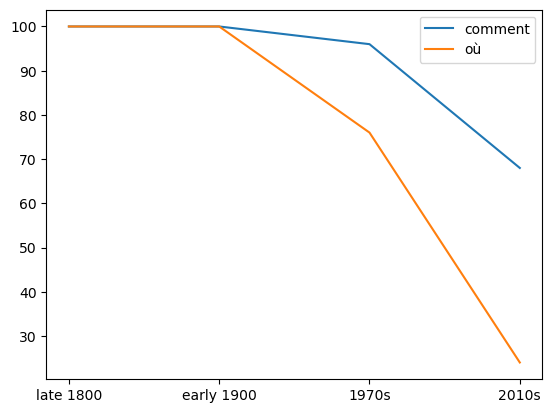
\includegraphics[width=10cm, height=6cm]{images/two.png}
    \end{center}
  
\end{frame}
%   FRAME END   --==-=-=-=-=-=-=-=-=-=-=-=-=-=-=-=-=-=-=-=-=-=-=-=-=-=-=-=-=-=-=
%   FRAME START   -=-=-=-=-=-=-=-=-=-=-=-=-=-=-=-=-=-=-=-=-=-=-=-=-=-=-=-=-=-=-=
\begin{frame}[c]{From predominant wh-ex situ to predominant wh-in situ}

    \textbf{\textsc{the decline of wh-ex situ}} (all types combined)
    \begin{center}
        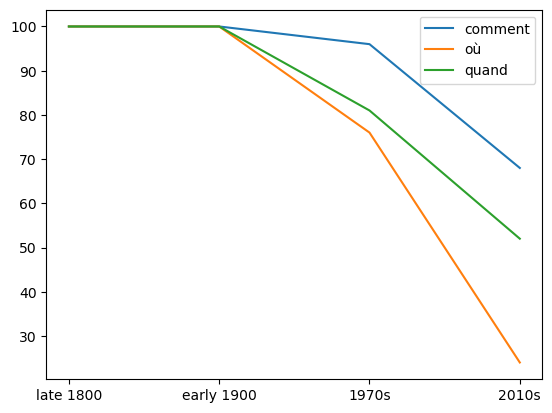
\includegraphics[width=10cm, height=6cm]{images/three.png}
    \end{center}
  
\end{frame}
%   FRAME END   --==-=-=-=-=-=-=-=-=-=-=-=-=-=-=-=-=-=-=-=-=-=-=-=-=-=-=-=-=-=-=
%   FRAME START   -=-=-=-=-=-=-=-=-=-=-=-=-=-=-=-=-=-=-=-=-=-=-=-=-=-=-=-=-=-=-=
\begin{frame}[c]{From predominant wh-ex situ to predominant wh-in situ}

    \textbf{\textsc{the decline of wh-ex situ}} (all types combined)
    \begin{center}
        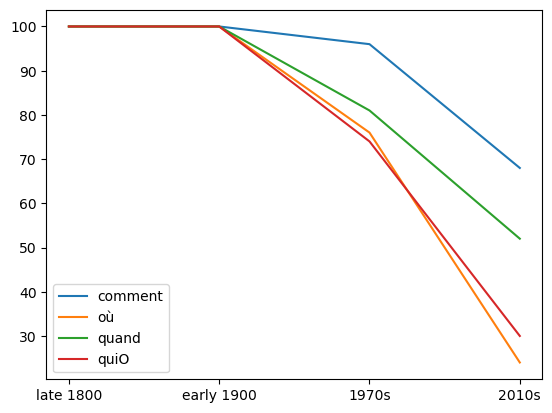
\includegraphics[width=10cm, height=6cm]{images/four.png}
    \end{center}
  
\end{frame}
%   FRAME END   --==-=-=-=-=-=-=-=-=-=-=-=-=-=-=-=-=-=-=-=-=-=-=-=-=-=-=-=-=-=-=
%   FRAME START   -=-=-=-=-=-=-=-=-=-=-=-=-=-=-=-=-=-=-=-=-=-=-=-=-=-=-=-=-=-=-=
\begin{frame}[c]{From predominant wh-ex situ to predominant wh-in situ}

    \textbf{\textsc{the decline of wh-ex situ}} (all types combined)
    \begin{center}
        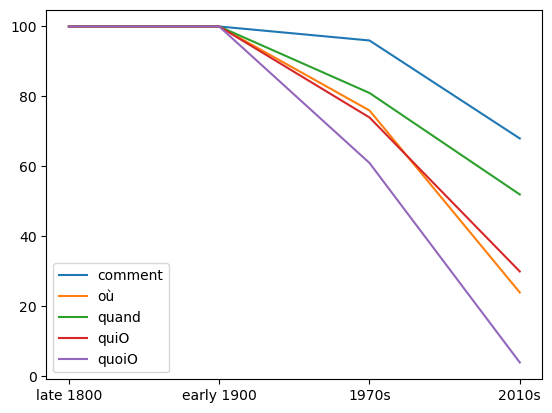
\includegraphics[width=10cm, height=6cm]{images/all.png}
    \end{center}
  
\end{frame}
%   FRAME END   --==-=-=-=-=-=-=-=-=-=-=-=-=-=-=-=-=-=-=-=-=-=-=-=-=-=-=-=-=-=-=
%   FRAME START   -=-=-=-=-=-=-=-=-=-=-=-=-=-=-=-=-=-=-=-=-=-=-=-=-=-=-=-=-=-=-=
\begin{frame}[c]{Towards predominant non-movement/activation}
  
\end{frame}
%   FRAME END   --==-=-=-=-=-=-=-=-=-=-=-=-=-=-=-=-=-=-=-=-=-=-=-=-=-=-=-=-=-=-=
%   FRAME START   -=-=-=-=-=-=-=-=-=-=-=-=-=-=-=-=-=-=-=-=-=-=-=-=-=-=-=-=-=-=-=
\begin{frame}[c]{From verb movement to predominant non-movement}
  
\end{frame}
%   FRAME END   --==-=-=-=-=-=-=-=-=-=-=-=-=-=-=-=-=-=-=-=-=-=-=-=-=-=-=-=-=-=-=
%=-=-=-=-=-=-=-=-=-=-=-=-=-=-=-=-=-=-=-=-=-=-=-=-=-=-=-=-=-=-=-=-=-=-=-=-=-=-=-=
\end{document}